\section{Move\_base} \label{sec:move_turtlebot}
To move the Turtlebot around in a hypermarket, the "move\_base" package is used. This package allows moving a mobile base to a desired goal in the world. By default recovery behaviours are performed when the robot is stuck which can be necessary as hypermarkets are semi-structured environment where many dynamic obstacles can be in the way. These behaviours are seen in figure \ref{fig:move_base}.\\

\begin{figure}[H]
    \centering
    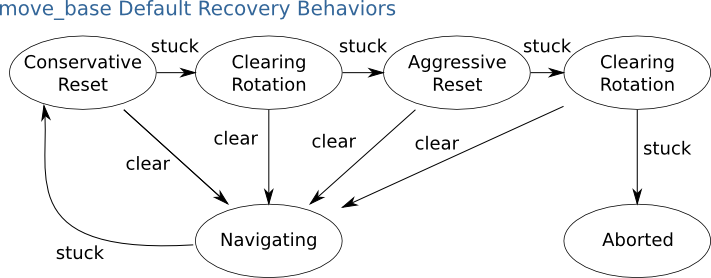
\includegraphics[width=0.9\textwidth]{figures/recovery_behaviors.png}
    \caption{Move\_base recovery behaviour.}
    \label{fig:move_base}
\end{figure}

The "move\_base" package allows the user to adjust many parameters the robot uses in its attempt to achieve a goal within a user-specified tolerance. These parameters can be changed on run-time using the parameter server. The "move\_base" package contains other key components for navigation like the "base\_local\_planner" package. This package uses algorithms connecting path planning to the robot by the use of a controller that generates velocity commands providing a map. The idea of these algorithms is as follow:

\begin{enumerate}
    \item Sample the linear velocities along x, y and the angular velocities along theta.
    \item Forward simulate each sampled velocity from the current state of the robot to predict the effect of applying this velocity for a period of time.
    \item The trajectories resulting of the forward simulation are scored according to different metrics that incorporates things such as distance to obstacle, goal and global path as well as speed. Trajectories that collide with obstacles are discarded.
    \item The trajectory with the highest score are chosen and the corresponding velocity is sent to the mobile base.
    \item Repeat.
\end{enumerate}

\begin{figure}[H]
    \centering
    \begin{minipage}[b]{0.57\linewidth}
    Figure \ref{fig:trajecories_mobileBase} shows trajectories simulated by a mobile base in order to determine which one has the highest score.\\
    Optionally, the "move\_base" package uses AMCL (Adaptive Monte Carlo Localisation) in order for the robot to localise itself in a map. This package uses filters to determine the pose of the robot in a known map.
    In order to keep a specific distance from the person being guided through the hypermarket, the velocity of the robot along with other metrics need to be changed dynamically.
    \end{minipage}
    \hspace{0.2cm}
    \begin{minipage}[b]{0.4\linewidth}
    \centering
    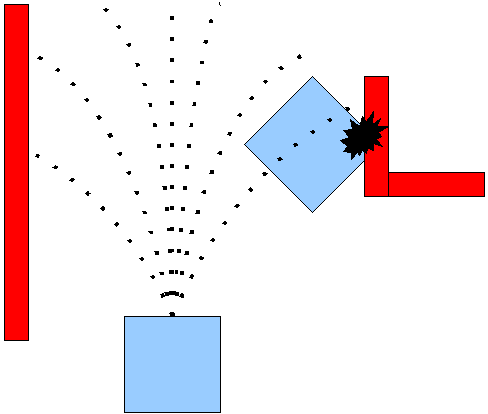
\includegraphics[width=\textwidth]{figures/local_plan.png}
    \caption{Mobile base with simulated trajectories to determine which path has the highest score.}
    \label{fig:trajecories_mobileBase}
    \end{minipage}
\end{figure}

The implemented node sends a goal to the action server by using an action client. This way of requesting the robot to move allows getting periodic feedback about the progress of the moving task, where three messages are used to communicate between the server and the client. These messages are Goal, Feedback and Result. In this case, the goal is a geometry message of type PoseStamped, that is defined by a position, orientation as well as a time stamp. The Feedback contains a PoseStamped message indicating the current pose of the robot in addition to GoalStatus message which is defined by unsigned integer values indicating the progress of the robot in completing the requested goal, being pending, active, aborted, succeeded or lost, among other status. The Result is GoalStatus message as well that is sent from the server to the client when the goal is completed, however, it is only sent once.\\

A graphical user interface were implemented by using a library called GTKMM to allow the customer to send a goal to the action server. The interface consists of 100 buttons with different labels indicating the different wares of the store, each buttons corresponds to a position on the map of the store. The buttons are arranged in a grid of 10 by 10 which is added to a scrolled window. The interface can be seen in figure \ref{fig:move_gui}.

\begin{figure}[H]
    \centering
    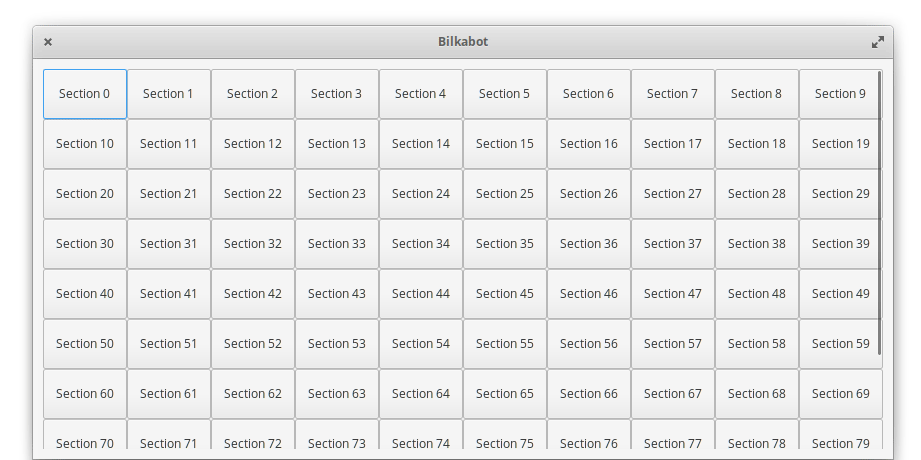
\includegraphics[width=0.9\textwidth]{figures/gtkmm_gui2.png}
    \caption{A graphical user interface showing different buttons that correspond to different wares of a store.}
    \label{fig:move_gui}
\end{figure}